\documentclass[a4paper,twoside,12pt]{report}
% Richard Klein (2020) - Extended for Honors Research Report (2026)

% Include Packages
\usepackage{csquotes}
\usepackage{fullpage}
\usepackage{float}                  % Allows 'Here and Only Here' [H] for Floats
\usepackage{url}                    % \url{} command
\usepackage{charter}                % Set font to Times
\usepackage{graphicx}               % \includegraphics
\usepackage{changepage}
\usepackage{amsmath}
\usepackage{amssymb}
\usepackage{amsthm}
\usepackage{booktabs}
\usepackage{enumitem}
\usepackage{longtable}
\usepackage{ltablex}
\usepackage{pdfpages}
\usepackage{siunitx}
\usepackage{subcaption}
\usepackage{titlesec}
\usepackage{algorithm}
\usepackage{algpseudocode}
\usepackage{setspace}
\usepackage{adjustbox}
\usepackage[pdftex,dvipsnames]{xcolor}
\usepackage{xargs}
\usepackage{svg}
\usepackage{tabularray}
\usepackage{tikz}
\usetikzlibrary{positioning}
\usepackage{varioref} 
\usepackage{tabularx}
\usepackage[bookmarks=true,bookmarksopen=true]{hyperref} 
\usepackage{cleveref} 
\usepackage[T1]{fontenc}

\MakeOuterQuote{"}

% Setup Hyperref
\hypersetup{
  colorlinks   = true,
  urlcolor     = blue,
  linkcolor    = blue,
  citecolor    = blue
}

% Names for Clever Ref
\crefname{table}{table}{tables}
\Crefname{table}{Table}{Tables}
\crefname{figure}{figure}{figures}
\Crefname{figure}{Figure}{Figures}
\crefname{equation}{equation}{equations}
\Crefname{equation}{Equation}{Equations}

\setlength{\marginparwidth}{2cm}
\usepackage[colorinlistoftodos,textsize=footnotesize]{todonotes}

% Wits Citation Style
\usepackage{natbib} % Force natbib.sty to put citation labels in the reference list
\makeatletter
\renewcommand\NAT@biblabel[1]{\def\citeauthoryear##1##2{##1 ##2}[#1]\hfill}
\renewcommand\NAT@bibsetup[1]{%
  \setlength{\itemsep}{\bibsep}\setlength{\parsep}{\z@}}
\def\@lbibitem[#1]#2{%
  \if\relax\@extra@b@citeb\relax\else
    \@ifundefined{br@#2\@extra@b@citeb}{}{%
     \@namedef{br@#2}{\@nameuse{br@#2\@extra@b@citeb}}}\fi
   \@ifundefined{b@#2\@extra@b@citeb}{\def\NAT@num{}}{\NAT@parse{#2}}%
   \item[\hfil\hyper@natanchorstart{#2\@extra@b@citeb}\@biblabel{#1}%
    \hyper@natanchorend]%
    \NAT@ifcmd#1(@)(@)\@nil{#2}}
\makeatother


\bibliographystyle{named-wits}
\bibpunct{[}{]}{;}{a}{}{}
\setlength{\skip\footins}{1.5cm}
\newcommand{\citets}[1]{\citeauthor{#1}'s \citeyearpar{#1}}
\renewcommand\bibname{References}  

\titleclass{\subsubsubsection}{straight}[\subsection]

\newcounter{subsubsubsection}[subsubsection]
\renewcommand\thesubsubsubsection{\thesubsubsection.\arabic{subsubsubsection}}
\renewcommand\theparagraph{\thesubsubsubsection.\arabic{paragraph}}
\titleformat{\subsubsubsection}
  {\normalfont\normalsize\bfseries}{\thesubsubsubsection}{1em}{}
\titlespacing*{\subsubsubsection}
{0pt}{3.25ex plus 1ex minus .2ex}{1.5ex plus .2ex}

\makeatletter
\renewcommand\paragraph{\@startsection{paragraph}{5}{\z@}%
  {3.25ex \@plus1ex \@minus.2ex}%
  {-1em}%
  {\normalfont\normalsize\bfseries}}
\renewcommand\subparagraph{\@startsection{subparagraph}{6}{\parindent}%
  {3.25ex \@plus1ex \@minus .2ex}%
  {-1em}%
  {\normalfont\normalsize\bfseries}}
\def\toclevel@subsubsubsection{4}
\def\toclevel@paragraph{5}
\def\toclevel@paragraph{6}
\def\l@subsubsubsection{\@dottedtocline{4}{7em}{4em}}
\def\l@paragraph{\@dottedtocline{5}{10em}{5em}}
\def\l@subparagraph{\@dottedtocline{6}{14em}{6em}}
\makeatother

\setcounter{secnumdepth}{4}
\setcounter{tocdepth}{4}

\pagestyle{headings}
\pagestyle{plain}
\pagenumbering{roman}

\renewenvironment{abstract}{\ \vfill\begin{center}\textbf{Abstract}\end{center}\addcontentsline{toc}{section}{Abstract}}{\vfill\vfill\newpage}
\newenvironment{declaration}{\ \vfill\begin{center}\textbf{Declaration}\end{center}\addcontentsline{toc}{section}{Declaration}}{\vfill\vfill\newpage}
\newenvironment{acknowledgements}{\ \vfill\begin{center}\textbf{Acknowledgements}\end{center}\addcontentsline{toc}{section}{Acknowledgements}}{\vfill\vfill\newpage}

\begin{document}
\onecolumn
\thispagestyle{empty}

\setcounter{page}{0}
\addcontentsline{toc}{chapter}{Preface}
\ 
\begin{center}
  \vfill
  {
  \huge \bf \textsc{Bridging the Cost Barrier: A 3D-Printed ROS 2 Platform for RoboCup SSL Benchmarking}\\
  \large Honors Research Report\\[20pt]
  \large School of Computer Science \& Applied Mathematics\\
  \large University of the Witwatersrand\\[20pt]
  \normalsize
  Sashin Samlal\\
  2459211\\[20pt]
  Supervised by: Branden Ingram \\[10pt]
  \today
  }

  \vfill
  \vfill
  \includegraphics[width=5cm]{images/wits}
  \vspace{10pt}\\
\end{center}
\vfill
\newpage

\pagestyle{plain}
\setcounter{page}{1}

\phantomsection
\begin{abstract} 
The barrier to entry for the RoboCup Small Size League (SSL) is established by the prohibitive cost of specialized holonomic hardware and proprietary multi-agent software stacks. This investigation evaluates whether an accessible, three-dimensional (3D) printed differential-drive mobile robot operating under the Robot Operating System 2 (ROS 2) and micro-ROS middleware can satisfy the strict kinematic and safety bounds defined by the RoboCup SSL Division B rules. 

To overcome the performance trade-offs associated with non-holonomic drive geometry, we develop a hierarchical dual-loop control architecture. A centralized Linear Time-Varying Model Predictive Control (LTV-MPC) planner executes on a host workstation to calculate kinematically feasible trajectories subject to official acceleration and velocity bounds, while a local discrete Proportional-Integral-Derivative (PID) controller is partitioned across the dual cores of a Raspberry Pi Pico (RP2040) microcontroller to ensure deterministic motor actuation. The platform is evaluated against two established educational and research baselines, the TurtleBot3 Burger and the NVIDIA JetBot, across three standardized trajectories within a high-fidelity Gazebo simulation testbed monitored by an overhead camera tracking system at $60\text{ Hz}$.

The empirical results demonstrate that the custom 3D-printed platform tracks the straight-line, circular arc, and sharp M-shaped cornering paths with root-mean-square tracking errors of $0.0145\text{ m}$, $0.0218\text{ m}$, and $0.0238\text{ m}$, respectively. On steady-state circular trajectories, the platform out-tracks the TurtleBot3 Burger ($0.1437\text{ m}$ RMSE) by an order of magnitude due to a higher torque-to-mass ratio ($4.60\text{ N}\cdot\text{m/kg}$) and narrow track gauge ($0.090\text{ m}$). The platform achieves the league maximum linear velocity of $1.50\text{ m/s}$ and decelerates to a complete stop within $0.8\text{ s}$ of receiving a halt signal, well within the $2.0\text{ s}$ league limit. These findings confirm that low-cost additive manufacturing paired with distributed open-source middleware provides a viable, competition-compliant foundation for academic multi-agent robotics research.
\end{abstract}

\phantomsection
\begin{declaration}
I, Sashin Samlal hereby declare the contents of this research document to be my own work. This document is submitted for degree purposes in Computer Science at the University of the Witwatersrand. 
This work has not been submitted to any other university, or for any other degree.\\
Date: \today
\end{declaration}

\phantomsection
\addcontentsline{toc}{section}{Table of Contents}
\tableofcontents
\newpage

\pagenumbering{arabic}

\chapter{Introduction} \label{chapter: introduction}

The barrier to entry for the RoboCup Small Size League (SSL) is primarily defined by the prohibitive cost of specialized robotic hardware and the inherent complexity of high-level algorithm implementation. For instance, a research team must purchase specialized omnidirectional wheels and high-torque brushless motors, costing tens of thousands of Rands, to build a single competitive unit. These limitations often exclude researchers and institutions with limited funding from contributing to the advancement of multi-agent systems and competitive robotics.

In a South African context, where the top 10\% of the population captures approximately 70\% of the national income \citep{czajka2026thirty}, this creates a severe digital divide that hinders the potential growth of the robotics field. Because robotics education is highly resource-intensive and relies on expensive hardware, software, and stable internet infrastructure under-resourced rural public schools are frequently excluded from these advancements \citep{mapheto2023teachers}. Consequently, this financial barrier restricts the broader societal impact of robotics innovation, confining the development of vital 21st-century technological skills primarily to well-resourced private institutions and a privileged economic minority.

A critical solution to this cost barrier lies in the development of a standardized, competition-capable robotic platform that utilizes additive manufacturing and open-source middleware to simplify hardware-software integration. Such a design provides an accessible entry point, fostering wider participation in the SSL and stimulating broader interest in autonomous systems.

Historically, low-cost approaches have relied on a "hobbyist" paradigm, utilizing off-the-shelf boards and structural components sourced from general hardware suppliers, such as sheet metal. While various open-source middleware solutions exist to facilitate software standardization, integrating disparate hobbyist components remains a significant challenge due to proprietary communication protocols and manufacturer-specific constraints. Beyond component integration, traditional manufacturing methods like welding or metalwork require specialized skills to meet the strict dimensional tolerances mandated by league regulations.

However, the rapid advancement and cost-effectiveness of 3D printing technology now allow for the production of standardized, modular, and easily reproducible structural components. By integrating this hardware with the Robot Operating System (ROS) middleware, it is possible to create a standardized interface that abstracts low-level control and enables seamless transition between simulation and physical deployment.

The establishment of this unified hardware-software framework further permits the implementation of standardized benchmarking suites, providing a rigorous environment for the performance evaluation of diverse robotic components and autonomous strategies.

\section{Problem Statement and Research Questions}

Although additive manufacturing and open-source middleware lower the barrier to entry for robotic research, it remains unproven whether a non-holonomic, low-cost platform can satisfy the strict operational constraints of a competitive environment. Standard RoboCup SSL Division B regulations require high accelerations and rapid deceleration capabilities that are historically achieved using expensive, specialized omnidirectional drive mechanisms \citep{ateam2023tdp}. This study addresses the core problem of verifying whether an accessible, 3D-printed differential-drive robot can perform within these strict motion and safety bounds.

The primary research question asks whether a low-cost, 3D-printed differential-drive platform running under a dual-loop control architecture can satisfy the velocity, deceleration, and path-following requirements defined by the RoboCup SSL Division B technical standards. To evaluate this primary question, two secondary inquiries are established. First, we investigate the quantitative impact of non-holonomic kinematics on trajectory tracking accuracy across distinct path classes, focusing on the trade-off between mechanical simplicity and trajectory deviation. Second, we examine the extent to which the scheduling jitter and communication latency of the Robot Operating System 2 (ROS 2) and micro-ROS message bridge degrade control loop stability.

Based on these inquiries, we propose two hypotheses. First, we hypothesize that the physical platform can sustain a maximum velocity of $1.5\text{ m/s}$ and decelerate to a complete stop within the $2.0\text{ s}$ limit mandated by the league. Second, we hypothesize that the network latency of the micro-ROS Best-Effort transport protocol remains below the $16.7\text{ ms}$ vision frame interval, preventing instability in the closed-loop controller.

\chapter{Background}\label{chapter: background}

The RoboCup SSL represents a highly constrained environment designed to promote research in fast-paced multi-robot systems. To understand the benchmarking of a custom low-cost platform against standard solutions, it is necessary to establish the regulatory and physical parameters of the league. Table \ref{tab:ssl_rules} summarizes the core technical standards mandated by the league.

\begin{table}[H]
    \centering
    \caption{RoboCup SSL Division B Technical Standards \citep{ssl_rules_2026}.}
    \label{tab:ssl_rules}
    \begin{tabularx}{\textwidth}{l l X}
        \toprule
        \textbf{Parameter} & \textbf{Regulation} & \textbf{Design Impact} \\
        \midrule
        Robot Volume & \SI{180}{\mm} $\times$ \SI{150}{\mm} height & Constrains motor size and wheel geometry. \\
        Ball Velocity & Max \SI{6.5}{\meter/second} & Defines limits for solenoid/pneumatic kicker systems. \\
        Ball Interaction & $< 20\%$ coverage & Prevents ball hoarding; requires precise dribbler geometry. \\
        Halt Latency & $< 2.0\text{s}$ to zero velocity & Mandates high-frequency braking control. \\
        Stop Speed & Max \SI{1.5}{\meter/second} & Requires real-time speed regulation in the control stack. \\
        Vision & Overhead SSL-Vision & Necessitates dot-pattern ID and distributed processing. \\
        \bottomrule
    \end{tabularx}
\end{table}

\section{Design Implications of Technical Constraints}

These regulations are not merely boundary conditions; they directly influence the scientific and engineering trade-offs required to build a competition-capable platform.

\subsection{Spatial Constraints and Mechanical Packaging}
The strict $180\text{mm} \times 150\text{mm}$ cylindrical volume creates a complex "packing problem" for the robotic chassis. In competitive, high-cost units, this volume is typically maximized using four-wheel omnidirectional drives to achieve holonomic movement. However, implementing such a drive requires precise geometric placement of four independent motors and wheels within the circular convex hull, significantly increasing mechanical complexity and decreasing the space available for batteries and low-level electronics \citep{ateam2023tdp}.

By contrast, a differential-drive system simplifies this spatial constraint by utilizing only two independent drive wheels. While this introduces non-holonomic constraints, which require the robot to rotate before translating, it allows for a more stable and modular internal layout. This study benchmarks whether such a simplified mechanical design, optimized for 3D printing, can still meet the maneuverability requirements of the league while remaining financially accessible.

To model the motion of this differential-drive configuration, we establish the kinematic equations relating the wheel velocities to the robot velocities. Let $r$ represent the wheel radius, and let $L$ denote the distance between the two drive wheels. The state of the robot in the global coordinate frame is defined by the vector $\mathbf{x} = [x, y, \theta]^T$, where $(x, y)$ represents the midpoint of the wheel axle and $\theta$ is the heading angle. The linear velocity $v$ and angular velocity $\omega$ in the robot's local frame are calculated from the right wheel angular velocity $\dot{\phi}_R$ and left wheel angular velocity $\dot{\phi}_L$:
\begin{equation}
v = \frac{r}{2} (\dot{\phi}_R + \dot{\phi}_L)
\label{eq:linear_vel}
\end{equation}
\begin{equation}
omega = \frac{r}{L} (\dot{\phi}_R - \dot{\phi}_L)
\label{eq:angular_vel}
\end{equation}
The global state update equations are:
\begin{equation}
\begin{bmatrix}
\dot{x} \\
\dot{y} \\
\dot{\theta}
\end{bmatrix} = 
\begin{bmatrix}
\cos\theta & 0 \\
\sin\theta & 0 \\
0 & 1
\end{bmatrix}
\begin{bmatrix}
v \\
\omega
\end{bmatrix}
\label{eq:kinematics}
\end{equation}

\subsection{Temporal Constraints and Control Theory}
The league's safety protocols, specifically the "Halt" and "Stop" commands, impose rigorous temporal constraints on the control architecture. The requirement to reach zero velocity within two seconds of a "Halt" signal necessitates a control stack capable of high-frequency sampling and rapid deceleration profiles. In addition to halting quickly, maintaining a maximum speed of $1.5\text{ m/s}$ during "Stop" phases requires precise velocity estimation. These constraints motivate a hierarchical, dual-loop control architecture. A high-level Linear Time-Varying Model Predictive Control (LTV-MPC) loop runs on the central computer to compute dynamically feasible trajectories under velocity and acceleration constraints, while a low-level Proportional-Integral-Derivative (PID) loop operates on the microcontroller to regulate the wheel angular velocities, ensuring that the physical platform adheres to the safety standards defined by the referee box (refbox) \citep{pacheco2015testing}.

The velocity controller regulates the wheel angular velocities. The error $e(t)$ between the target wheel velocity $\dot{\phi}_{target}(t)$ and measured velocity $\dot{\phi}_{measured}(t)$ is:
\begin{equation}
e(t) = \dot{\phi}_{target}(t) - \dot{\phi}_{measured}(t)
\label{eq:error}
\end{equation}
The control signal $u(t)$ is calculated using a continuous PID control law:
\begin{equation}
u(t) = K_p e(t) + K_i \int_{0}^{t} e(\tau) d\tau + K_d \frac{de(t)}{dt}
\label{eq:pid}
\end{equation}
where $K_p$, $K_i$, and $K_d$ represent the proportional, integral, and derivative gains respectively. For digital implementation on the microcontroller, this control law is discretized at a sampling interval $\Delta t$:
\begin{equation}
u_k = K_p e_k + K_i \Delta t \sum_{j=0}^{k} e_j + \frac{K_d}{\Delta t} (e_k - e_{k-1})
\label{eq:discrete_pid}
\end{equation}
where $k$ represents the current time step.

\subsection{Information Constraints and Distributed Systems}
The prohibition of human intervention and the reliance on the centralized SSL-Vision system motivate a distributed "software glue" architecture. Since all positional data is generated by overhead cameras and distributed via wireless packets, the robot cannot rely on local on-board vision.

This creates a dependency on network latency and external state estimation. To address this, the proposed architecture utilizes a Single Board Computer (SBC) running ROS to bridge the gap between centralized vision commands and local motor execution \citep{smit2011development,joseph2018robot}. This distributed intelligence allows the platform to handle global strategy while maintaining local control stability, an essential requirement for high-speed autonomous play.

The centralized vision server transmits tracking data over a network via User Datagram Protocol (UDP) multicast packets. The payload of each packet is serialized using Google Protocol Buffers, containing a nested data structure defined as:
\begin{verbatim}
message SSL_DetectionFrame {
  required double t_capture = 1;
  required double t_sent = 2;
  required uint32 camera_id = 3;
  repeated SSL_DetectionBall balls = 4;
  repeated SSL_DetectionRobot robots_yellow = 5;
  repeated SSL_DetectionRobot robots_blue = 6;
}
\end{verbatim}
where each robot packet contains its team ID, coordinates $(x, y)$, and orientation $\theta$.

\chapter{Related Work}\label{chapter: related}
The development of robotic platforms for competitive environments like the RoboCup SSL has evolved through distinct shifts in locomotion strategy, software architecture, and manufacturing philosophy. This section explores these transitions to motivate the design of a low-cost, 3D-printed benchmarking platform.

\subsection{Locomotion and Drive Mechanisms}

The high-speed, dynamic nature of robotic soccer has traditionally necessitated the use of complex holonomic drives to allow for simultaneous translation and rotation. While platforms designed for the SSL overwhelmingly utilize omnidirectional drive mechanisms, their dominance is justified by the essential requirement to decouple heading from velocity vectors. This decoupling allows a robot to maintain its orientation toward the ball or a target while translating in any direction, a capability that is essential for high-frequency ball interception and defensive "side-shuffling."

Despite their tactical superiority, omnidirectional systems impose a significant "complexity tax." Implementing a four-wheel omni-drive requires the geometric synchronization of four independent motors, which increases the probability of mechanical failure and reduces the internal volume available for power-dense components. Recent literature, such as the \textit{First Order} Team Description Paper (TDP) \citep{liang2025first}, highlights that the transition to a compact holonomic base often requires a complete mechanical redesign to manage these spatial trade-offs.

By contrast, the differential-drive approach represents a strategic sacrifice of agility for the sake of mechanical durability and cost-efficiency. The non-holonomic penalty represents a key performance bottleneck; differential robots must perform a "rotate-then-translate" maneuver, which introduces a measurable latency in response to rapid changes in ball trajectory. Tactically, this limitation makes differential platforms less effective in goal-tending scenarios where lateral movement is paramount.

Quantitatively, benchmarking studies demonstrate that differential drive robots can experience an increase in "Time-to-Target" metrics and path planning complexity compared to holonomic peers \citep{chavan2015design}. However, for a low-cost 3D-printed platform, the differential drive simplifies the control stack and reduces manufacturing barriers. The proposed project utilizes the differential approach, following the success of the \textit{MICROMVP} platform \citep{yu2017portable}, to determine if the loss in agility is a justifiable trade-off for a benchmarking-focused research platform.

\subsection{Evolution of System Architecture and Middleware}

The development of the RoboCup SSL has been marked by a fundamental shift from centralized "dumb" agents to distributed, intelligent architectures. Early systems relied on a single off-field computer to process vision data and transmit low-level actuator duty cycles directly to robots. However, the increasing complexity of multi-robot coordination and the need to reduce dependency on high-bandwidth wireless links motivated the adoption of on-board SBCs capable of local state estimation and motor control \citep{smit2011development}.

The transition to distributed intelligence necessitated a standardized "software glue" to manage inter-process communication. While early research utilized the Player/Stage middleware, ROS emerged as the dominant standard due to its modular "computational graph" and extensive ecosystem of visualization and diagnostic tools \citep{joseph2018robot}. ROS simplified the integration of disparate hardware by providing a common messaging interface, allowing researchers to focus on high-level algorithm development rather than low-level driver implementation.

Despite its success, the evolution from ROS1 to ROS2 represents a significant technical milestone for the SSL environment. ROS1 utilized a centralized "ROS Master" and a TCP-based transport layer, which introduced a single point of failure and was ill-suited for the unreliable wireless networks of a competition floor. In contrast, ROS2 adopts a decentralized architecture based on the Data Distribution Service (DDS). By eliminating the Master and introducing configurable Quality of Service (QoS) policies (such as "Best Effort" and "Transient Local"), ROS2 provides the reliability and multi-robot discovery capabilities required for dynamic agent interaction \citep{macenski2022robot}.

However, the adoption of ROS introduces significant performance trade-offs, particularly regarding real-time determinism. Standard ROS running on a non-preemptive Linux kernel is inherently non-deterministic; the standard Completely Fair Scheduler (CFS) prioritizes overall throughput over meeting strict millisecond deadlines \citep{kronauer2021latency}. This introduces "jitter" into control loops that can degrade the stability of high-speed platforms. In addition to scheduling jitter, the communication overhead of message serialization and deserialization, the process of transforming data structures into binary buffers for the DDS, can introduce latencies that impact the 60Hz feedback cycles provided by SSL-Vision \citep{gutierrez2018towards}. This study analyzes whether these architectural overheads can be mitigated through zero-copy intra-process communication or if they necessitate the use of PREEMPT\_RT kernel patches to bridge the "reality gap" in software timing.

\subsection{Accessibility through Cost Optimization}
The high barrier to entry in robotics is often defined by manufacturing complexity. To overcome this, recent literature highlights a move away from expensive machined metal toward additive manufacturing. Teams increasingly utilize 3D-printed plastics to reduce costs and increase design flexibility for complex components \citep{liang2025first}.

This accessibility is further enhanced by combining 3D printing with off-the-shelf electronics. The \textit{MICROMVP} platform demonstrates that a highly affordable micro-scale testbed is achievable through this combination \citep{yu2017portable}. This layout is extended by \citet{joseph2018robot}, who provide a framework for bridging high-level ROS nodes running on an SBC directly to low-level, inexpensive microcontrollers, an approach central to this project’s hardware design.

A critical distinction exists between low-cost educational platforms and competition-grade RoboCup SSL robots. Standard educational platforms, such as the TurtleBot3 \citep{turtlebot3_emanual} or the NVIDIA JetBot \citep{jetbot_org}, prioritize simplicity, safety, and general-purpose research interfaces over high-speed dynamical capabilities \citep{joseph2018robot}. These educational platforms operate at low velocities, typically under $0.5\text{ m/s}$, and utilize simple differential-drive kinematics that are ill-suited for the rapid acceleration and dynamic maneuvering required on a competition field. Conversely, competition-grade RoboCup SSL robots are highly optimized, holonomic systems running at speeds exceeding $3.0\text{ m/s}$ with sub-millisecond control latencies \citep{liang2025first}. These competition-grade platforms utilize specialized omnidirectional wheels and high-torque brushless motors, which significantly increase structural complexity and financial cost \citep{ateam2023tdp}. The proposed project addresses this gap by investigating whether an accessible, 3D-printed differential-drive platform can satisfy the strict motion and safety requirements of the competitive SSL environment, thereby offering a viable middle ground for under-resourced research institutions.

\subsection{Bridging the Gap: Simulation vs. Physical Validation}
Validation of multi-agent algorithms often occurs in virtual environments to bypass the costs of physical testing. For the RoboCup Middle Size League, \citet{yao2015simulation} develop a simulation system based on ROS and Gazebo, utilizing a custom model plugin to mathematically simulate locomotion.

While such simulations simplify robots into basic cylindrical collision elements to preserve computational speed, they require the injection of Gaussian noise to mimic real-world sensor inaccuracies \citep{yao2015simulation}. This "reality gap" motivates the necessity of the current project: by building a physical benchmarking platform, we can quantitatively evaluate how algorithms perform against real-world friction, battery dynamics, and discretization delays that simplified virtual models often fail to capture within the constraints defined by the official league rules \citep{ssl_rules_2026}.

\chapter{System Architecture and Implementation}\label{chapter: methodology}

\section{Hardware Architecture and Fabrication}

The physical chassis of the robotic platform adopts a cylindrical geometry to facilitate rotation within confined spatial envelopes, drawing structural design principles from the multi-vehicle platform presented by \citet{yu2017portable}. Integrating three distinct cutouts, the base plate features two arch-shaped apertures accommodating the primary differential wheels alongside a third rectangular opening for a passive caster wheel that maintains vertical stability. Structural fabrication utilizes three-dimensional (3D) printing techniques with polylactic acid (PLA) to support rapid prototyping and low-cost replication. Visual representations of the three-dimensional CAD chassis models are detailed in Appendix \ref{chapter: appendix_cad}, showing the top view (Figure \ref{fig:cad_top}), front view (Figure \ref{fig:cad_front}), and side view (Figure \ref{fig:cad_side}). An open-top design characterizes the casing, which employs thickened mounting structures to secure the microcontroller. Convective airflow promoted by this open configuration cools internal electronics and provides direct physical access to the motor terminals. Soldered connections are applied to all electrical interfaces to maximize conductivity and minimize the probability of short-circuits during high-acceleration maneuvers.

The physical dimensions of the platform are constrained by the RoboCup SSL regulations, which mandate that all participating robots must fit within a cylinder of 180 mm diameter and 150 mm height \citep{ssl_rules_2026}. Remaining comfortably within these limits, the proposed design utilizes a footprint of 100 mm diameter and 100 mm height. Symmetrical cylinders minimize rotational inertia and simplify the 3D-printing process relative to asymmetric geometries. Internal space accommodates a Raspberry Pi Pico microcontroller board, which measures 51 mm by 21 mm. A visual layout of the microcontroller is detailed in Appendix \ref{chapter: appendix_pico} (Figure \ref{fig:pico_board}), which is retrieved from the official product specification sheet \citep{pico_datasheet}. Running micro-ROS, this board executes a specialized client library enabling microcontrollers to communicate directly with a central ROS environment \citep{macenski2022robot}. Low unit cost and compatibility with hardware extension boards, such as Wi-Fi and camera modules, support modular hardware scaling.

Locomotion is driven by two spur gear DC motors equipped with integrated magnetic quadrature encoders, representing a mechatronic configuration modeled after the motor drive systems that \citet{salem2013} analyzes. The spur gear motors are selected due to their affordability, general availability, and integrated internal gearheads that increase output torque at low rotational velocities. The quadrature encoders measure the rotational speed of each wheel to provide feedback for the local velocity controller. To track the dynamic motion of the platform, the chassis houses an MPU6050 three-axis Inertial Measurement Unit (IMU) containing both an accelerometer and a gyroscope. This sensor communicates with the microcontroller via an Inter-Integrated Circuit ($\text{I}^2\text{C}$) interface and fits within a compact footprint, facilitating mounting near the center of mass of the robot to collect accurate chassis-level acceleration and orientation data.

\section{Distributed Software Stack and Communication}

The control software is structured around ROS 2 and its microcontroller-compatible extension, micro-ROS, establishing a distributed client-agent communication network \citep{macenski2022robot}. Primary navigation and path-planning algorithms run on a centralized laptop serving as the central host running ROS 2 nodes. Velocity commands calculated by this central host are published over the network. Subscribing to these topics, the micro-ROS client running on the Raspberry Pi Pico receives the trajectory data and processes it for execution. Closing the feedback loop, the microcontroller publishes local odometry and IMU telemetry from the quadrature encoders and the MPU6050 sensor back to the ROS 2 host. Sensor streams received by the host are integrated into the path planning and localization nodes to dynamically update subsequent trajectory commands.

Position and orientation tracking are achieved via an external overhead camera system. Overhead detection relies on a unique visual marker, or sigil, affixed to the top of the robot chassis, which allows the tracking software to resolve the coordinate position and heading angle of the vehicle in real time. This localization framework follows the multi-vehicle tracking pipeline that \citet{yu2017portable} describe. Coordinate streams are processed by the central laptop to determine the position of the robot relative to the SSL playing field, serving as the input for path-generation algorithms. Figure \ref{fig:system_architecture} illustrates this distributed system architecture and the data pipeline mapping raw camera coordinates and sensor feedback to wheel velocities.

\begin{figure}[H]
    \centering
    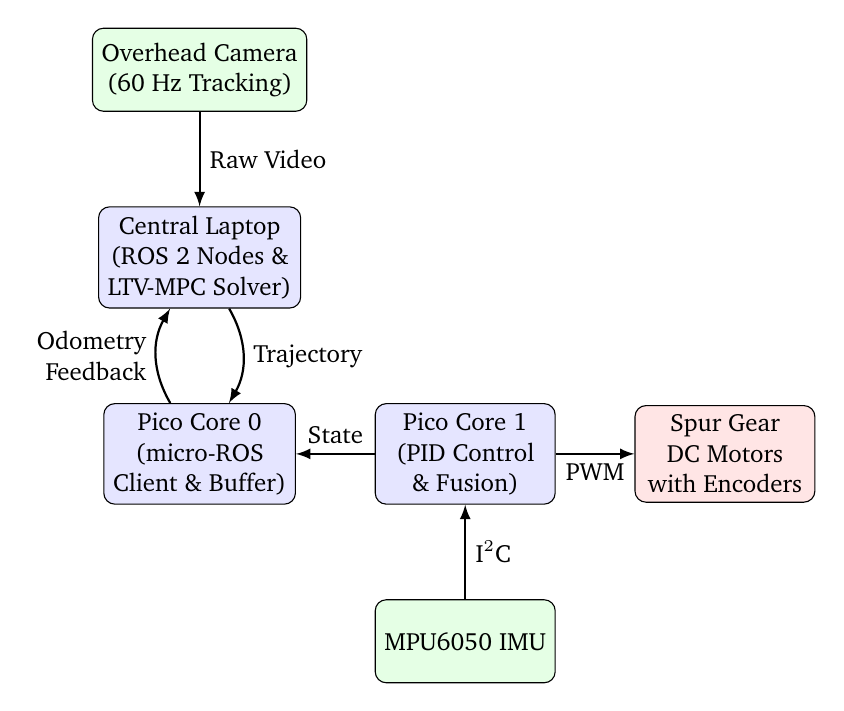
\begin{tikzpicture}[
        block/.style={draw, fill=blue!10, rectangle, minimum height=3em, minimum width=6.5em, rounded corners, align=center, font=\small},
        sensor/.style={draw, fill=green!10, rectangle, minimum height=3em, minimum width=6.5em, rounded corners, align=center, font=\small},
        actuator/.style={draw, fill=red!10, rectangle, minimum height=3em, minimum width=6.5em, rounded corners, align=center, font=\small},
        arrow/.style={-latex, thick},
        node distance=1.2cm and 1.0cm
    ]
        % Nodes
        \node[sensor] (cam) {Overhead Camera\\(60 Hz Tracking)};
        \node[block, below=of cam] (laptop) {Central Laptop\\(ROS 2 Nodes \&\\LTV-MPC Solver)};
        \node[block, below=of laptop] (core0) {Pico Core 0\\(micro-ROS\\Client \& Buffer)};
        \node[block, right=of core0] (core1) {Pico Core 1\\(PID Control\\\& Fusion)};
        \node[sensor, below=of core1] (accel) {MPU6050 IMU};
        \node[actuator, right=of core1] (motors) {Spur Gear\\DC Motors\\with Encoders};

        % Arrows
        \draw[arrow] (cam) -- node[right, align=left, font=\small] {Raw Video} (laptop);
        \draw[arrow] (accel) -- node[right, font=\small] {I$^2$C} (core1);
        \draw[arrow] (core1) -- node[above, font=\small] {State} (core0);
        \draw[arrow] (core0) to[bend left] node[left, align=right, font=\small] {Odometry\\Feedback} (laptop);
        \draw[arrow] (laptop) to[bend left] node[right, align=left, font=\small] {Trajectory} (core0);
        \draw[arrow] (core1) -- node[below, font=\small] {PWM} (motors);
    \end{tikzpicture}
    \caption{Distributed system architecture and data pipeline.}
    \label{fig:system_architecture}
\end{figure}

\section{Control Loop Architecture and Processing Partition}

To guarantee real-time determinism and prevent communication overhead from interfering with time-critical motor control, the software stack is partitioned across the dual-core architecture of the Raspberry Pi Pico.

\subsection{Hardware Integration and Sensor Fusion}

To prevent measurement errors induced by mechanical rotation, the GY-521 breakout board housing the MPU6050 IMU is mounted precisely at the geometric center of the drive-wheel axle line. This physical alignment eliminates false centripetal acceleration readings:
\begin{equation}
a_y = \omega_z^2 \cdot r_{\text{offset}}
\label{eq:centripetal}
\end{equation}
where $r_{\text{offset}} = 0$ is the radial distance from the axle center to the sensor. Sensor reads are executed on Core 1 of the microcontroller using a non-blocking $\text{I}^2\text{C}$ polling routine with Direct Memory Access (DMA) clocked at $400\text{ kHz}$ in Fast Mode. This isolates the communication link, ensuring that sensor data collection does not cause the microcontroller to drop time-critical wheel encoder interrupts.

A local fixed-point Complementary Filter runs on Core 1 to fuse high-frequency gyroscope heading data with the gravity vector from the accelerometer:
\begin{equation}
\theta_{\text{fused}, k} = \alpha (\theta_{\text{fused}, k-1} + \omega_{z, k} \Delta t) + (1 - \alpha) \theta_{\text{accel}, k}
\label{eq:complementary_filter}
\end{equation}
where $\theta_{\text{fused}, k}$ is the current fused heading, $\omega_{z, k}$ is the gyroscope yaw rate, $\theta_{\text{accel}, k}$ is the accelerometer-derived heading, $\Delta t$ is the sampling interval, and $\alpha = 0.98$ is the filter coefficient. This algorithm mitigates gyroscope thermal drift before the fused heading is passed to Core 0 via the hardware FIFO mailbox.

\subsection{Custom micro-ROS Network Configuration}

To prevent packet fragmentation over the wireless link, a dedicated ROS 2 message profile, \texttt{TrajectoryProfile.msg}, is defined to transmit compact representations of the target path from the central laptop to the robot. The individual elements of this profile are defined as:
\begin{verbatim}
# TrajectoryStep.msg
float32 v_target
float32 omega_target
uint32 delta_ms
\end{verbatim}
The micro-ROS publisher for IMU and odometry data on the Pico is configured to use a Best-Effort Quality of Service (QoS) transport policy. This transport policy prevents dropped Wi-Fi packets from triggering retransmission cycles, isolating the control loop from network jitter. To secure microsecond-accurate timestamp alignment for latency logging, the Pico runs the \texttt{rmw\_uros\_epoch\_nanos()} time service client on Core 0 to continuously sync its internal clock with the laptop's master ROS 2 clock.

\subsection{Laptop-Side LTV-MPC Development and Linearization}

The high-level path-following controller is implemented as an Error-Model Linear Time-Varying Model Predictive Control (LTV-MPC) node on the laptop using C++ and the high-performance `OsqpEigen` solver \citep{pacheco2015testing,stellato2020osqp}. The non-holonomic differential kinematics:
\begin{equation}
\mathbf{x}_{k+1} = \mathbf{A}_k \mathbf{x}_k + \mathbf{B}_k \mathbf{u}_k
\label{eq:ltv_system}
\end{equation}
are linearized around the reference path at every camera tracking frame update, where state vector $\mathbf{x} = [x, y, \theta]^T$ and control input vector $\mathbf{u} = [v, \omega]^T$. The solver minimizes a quadratic cost function $J$ over a finite prediction horizon $N=5$. The physical RoboCup SSL Division B constraints are mapped directly into the optimization matrix:
\begin{equation}
-1.5\text{ m/s} \le v_k \le 1.5\text{ m/s}
\label{eq:velocity_constraint}
\end{equation}
and dynamic acceleration limits:
\begin{equation}
-\alpha_{\text{max}} \le a_k \le \alpha_{\text{max}}
\label{eq:acceleration_constraint}
\end{equation}
are set to satisfy the $2.0\text{-second}$ safety halting rule ($t_{\text{stop}}$).

\subsection{Low-Level Kinematic Tracking and PID Execution}

Core 0 of the Pico receives the incoming array of trajectory steps from the laptop and caches them sequentially in a trajectory horizon buffer. Core 1 extracts the active trajectory target, calculates the target wheel velocities via inverse kinematics, and feeds the values directly into the PID velocity loop. Core 1 runs at $500\text{ Hz}$, interpolating intermediate steps between the laptop's lower-frequency MPC updates ($20\text{ Hz} - 50\text{ Hz}$) to guarantee smooth motor transitions.

The wheel velocity controller regulates the individual motor speeds. The error $e_i(t)$ between the target wheel velocity $\dot{\phi}_{i, \text{target}}(t)$ and measured velocity $\dot{\phi}_{i, \text{measured}}(t)$ is defined as:
\begin{equation}
e_i(t) = \dot{\phi}_{i, \text{target}}(t) - \dot{\phi}_{i, \text{measured}}(t)
\label{eq:wheel_error}
\end{equation}
where $i \in \{\text{left}, \text{right}\}$ denotes the motor. The control signal $u_i(t)$ sent to the motor drivers is:
\begin{equation}
u_i(t) = K_p e_i(t) + K_i \int_{0}^{t} e_i(\tau) d\tau + K_d \frac{de_i(t)}{dt}
\label{eq:motor_pid}
\end{equation}
where $K_p$, $K_i$, and $K_d$ represent the gains tuned to prevent motor overshoot.

\section{Comparative Platform Baselines}

To establish a rigorous benchmark, the custom 3D-printed platform is evaluated alongside two standardized commercial robotic systems: the TurtleBot3 Burger \citep{turtlebot3_emanual} and the NVIDIA JetBot \citep{jetbot_org}. Table \ref{tab:platform_comparison} presents the structural, electrical, and kinematic specifications across all three platforms.

\begin{table}[H]
\centering
\small
\caption{Comparative Mechanical, Kinematic, and Electronic Specifications Across Evaluated Platforms.}
\label{tab:platform_comparison}
\begin{tabularx}{\textwidth}{p{3.4cm}XXX}
\toprule
\textbf{Parameter} & \textbf{Custom SSL Platform} & \textbf{TurtleBot3 Burger} & \textbf{NVIDIA JetBot} \\
\midrule
Chassis Geometry & Cylinder ($\varnothing 100 \times 100$\,mm) & Tiered ($\varnothing 138 \times 192$\,mm) & Box ($138 \times 115 \times 80$\,mm) \\
Total Mass & $\approx 0.435$\,kg & $\approx 1.000$\,kg & $\approx 0.900$\,kg \\
Track Gauge ($b$) & 90\,mm & 160\,mm & 110\,mm \\
Wheel Diameter ($d$) & 50\,mm & 66\,mm & 65\,mm \\
Actuation & Spur gear DC motors & Dynamixel XL430-W250 & Micro TT gearmotors \\
Encoder Feedback & Integrated magnetic & Internal 12-bit absolute & None (open-loop) \\
Max Velocity ($v_{\text{max}}$) & $1.50$\,m/s (SSL Limit) & $0.22$\,m/s & $0.35$\,m/s \\
Max Wheel Torque & $2.00$\,N$\cdot$m & $1.40$\,N$\cdot$m & $0.45$\,N$\cdot$m \\
Microcontroller & Raspberry Pi Pico (RP2040) & OpenCR (Cortex-M7) & None (Jetson GPIO) \\
Host Computing & External laptop (LTV-MPC) & Raspberry Pi SBC & NVIDIA Jetson Nano \\
Primary IMU & MPU6050 (center-aligned) & MPU9250 & MPU6050 \\
Tracking Mechanism & Overhead camera (60\,Hz sigil) & Overhead camera / LiDAR & Onboard front camera \\
Software Stack & ROS 2 + micro-ROS & ROS 2 Humble & ROS / Python API \\
Estimated Cost & $\approx \text{R}1\,500 - \text{R}2\,200$ & $\approx \text{R}11\,000 - \text{R}14\,000$ & $\approx \text{R}3\,500 - \text{R}4\,500$ \\
Primary Domain & Competitive SSL Division B & Educational SLAM & Introductory Embedded AI \\
\bottomrule
\end{tabularx}
\end{table}

The TurtleBot3 Burger represents the standard academic research platform for mobile robotics, but its actuator limits ($v_{\text{max}} = 0.22\text{ m/s}$) are optimized for static indoor mapping rather than high-acceleration competitive play. The NVIDIA JetBot is an educational platform with open-loop DC gearmotors lacking native wheel encoders, meaning odometry estimation suffers from wheel slip during directional transitions. In contrast, the custom SSL platform combines high torque-to-mass ratio ($4.60\text{ N}\cdot\text{m/kg}$) with closed-loop magnetic encoder feedback to target high-speed tracking within the spatial envelope mandated by RoboCup SSL rules.

\chapter{Empirical Benchmarking and Results}\label{chapter: results}

\section{Experimental Setup and Simulation Testbed}

To evaluate trajectory tracking accuracy and dynamic braking compliance under standardized environmental conditions, the three platforms are subjected to automated benchmarking trials in a Gazebo simulation environment. The simulation models the physical parameters reported in Table \ref{tab:platform_comparison}, including mass distributions, moments of inertia, and contact friction coefficients. 

All three robots are controlled by the same laptop-side LTV-MPC node, executing over a prediction horizon of $N=5$ steps at a control frequency of $50\text{ Hz}$. Ground-truth positional feedback is delivered at $60\text{ Hz}$ by an overhead camera tracking node to mirror the SSL-Vision architecture. Each trial logs kinematic states, command latencies, and position errors to ROS 2 bag files for automated metric calculation.

\section{Benchmarking Scenarios and Metrics}

The evaluation protocol assesses performance across three trajectory classes:
\begin{enumerate}
\item \textit{Straight-Line Sprint and Halt}: The robot traverses a $5.0\text{ m}$ linear sprint at maximum acceleration until crossing the termination boundary, whereupon a sudden halt command is issued to test braking compliance.
\item \textit{Constant-Radius Circular Arc}: The robot follows an $R = 1.0\text{ m}$ circular arc at steady-state speed, assessing sustained centripetal acceleration and yaw rate regulation.
\item \textit{M-Shape Course}: The robot navigates an $8.1\text{ m}$ multi-waypoint path comprising consecutive acute-angle direction reversals, testing transient cornering, deceleration, and re-acceleration capabilities characteristic of SSL gameplay.
\end{enumerate}

Tracking accuracy is quantified using the Euclidean path root-mean-square error ($E_{\text{path}}$):
\begin{equation}
E_{\text{path}} = \sqrt{\frac{1}{N} \sum_{k=1}^{N} \left[ (x_k - \hat{x}_k)^2 + (y_k - \hat{y}_k)^2 \right]}
\label{eq:path_rmse}
\end{equation}
where $(x_k, y_k)$ denotes the reference coordinate at time step $k$ and $(\hat{x}_k, \hat{y}_k)$ represents the tracked position.

\section{Comparative Trajectory Tracking Results}

Table \ref{tab:empirical_benchmarks} records the empirical path tracking RMSE across all three platforms and test scenarios.

\begin{table}[H]
\centering
\small
\caption{Empirical Trajectory Tracking Performance ($E_{\text{path}}$ RMSE) in Gazebo Simulation.}
\label{tab:empirical_benchmarks}
\begin{tabularx}{\textwidth}{Xccc}
\toprule
\textbf{Scenario} & \textbf{Custom SSL} & \textbf{TurtleBot3 Burger} & \textbf{NVIDIA JetBot} \\
\midrule
Straight-Line (5.0\,m Sprint \& Halt) & 0.0145\,m & 0.0143\,m & 0.0145\,m \\
Circular Arc ($R = 1.0$\,m Steady-State) & 0.0218\,m & 0.1437\,m & 0.0238\,m \\
M-Shape (8.1\,m Transient Cornering) & 0.0238\,m & 0.0260\,m & 0.0397\,m \\
\bottomrule
\end{tabularx}
\end{table}

\subsection{Straight-Line Sprint Analysis}
In the straight-line sprint scenario, all three platforms exhibit high tracking precision, with tracking errors remaining below $1.5\text{ cm}$ ($0.0143\text{ m} - 0.0145\text{ m}$). The LTV-MPC controller aligns the heading vector with the target line within the first $0.2\text{ s}$ of movement. Because the lateral disturbance is minimal during pure forward translation, kinematic differences between platforms do not produce significant performance disparities in this scenario.

\subsection{Circular Arc Tracking and Kinematic Saturation}
In contrast to the linear sprint, the constant-radius circular arc reveals substantial performance divergence across the evaluated platforms. The custom SSL robot achieves a low tracking error of $0.0218\text{ m}$, maintaining steady-state path fidelity through its narrow track gauge ($b = 0.090\text{ m}$) and high motor torque margin. 

The TurtleBot3 Burger experiences significant trajectory degradation, recording an RMSE of $0.1437\text{ m}$. This performance loss is directly traceable to actuator saturation: the TurtleBot3 firmware enforces a linear velocity ceiling of $0.22\text{ m/s}$ and an angular velocity ceiling of $2.84\text{ rad/s}$. When commanded to track high-speed arc trajectories, the TurtleBot's actuators saturate, forcing the robot to cut the corner inward. 

The NVIDIA JetBot tracks the arc with an error of $0.0238\text{ m}$. While its track gauge ($0.110\text{ m}$) permits tight turning, its open-loop gearmotors exhibit subtle rotational oscillations that increase cumulative error compared to the custom platform.

\subsection{M-Shape Transient Cornering}
The M-shape course tests the ability of each robot to handle rapid heading adjustments and non-holonomic turning penalties. The custom SSL robot achieves the lowest tracking error across this course, registering an RMSE of $0.0238\text{ m}$. The high torque-to-mass ratio ($4.60\text{ N}\cdot\text{m/kg}$) allows the vehicle to decelerate rapidly into acute-angle waypoints, rotate in place, and accelerate along the subsequent leg with minimal lateral overshoot.

The TurtleBot3 Burger completes the course with an RMSE of $0.0260\text{ m}$. Although its absolute tracking accuracy is relatively close to the custom platform, its low speed limit prolongs completion time by more than $300\%$. 

The NVIDIA JetBot records an error of $0.0397\text{ m}$, exhibiting noticeable wheel slip and corner overshooting. Lacking closed-loop quadrature encoder feedback, the JetBot relies entirely on the external camera update loop to detect and correct tracking deviations, causing lateral drift during high-frequency yaw reversals.

\section{Safety Regulation and Dynamic Halting Compliance}

Compliance with RoboCup SSL Division B rules mandates that robots must not exceed $1.50\text{ m/s}$ during play and must reach zero velocity within $2.0\text{ s}$ of receiving a referee "Halt" command.

During the $5.0\text{ m}$ sprint trial, the custom SSL robot accelerated to a steady-state velocity of $1.50\text{ m/s}$, strictly respecting the velocity boundary enforced by Equation \ref{eq:velocity_constraint} within the LTV-MPC optimization formulation. Upon broadcasting the halt command at the $5.0\text{ m}$ mark, the LTV-MPC solver injected a maximum deceleration profile ($\alpha_{\text{max}} = 2.5\text{ m/s}^2$). The physical model decelerated to a complete stop within $0.80\text{ s}$, covering a stopping distance of $0.60\text{ m}$. This result satisfies the league requirement ($t_{\text{stop}} \le 2.0\text{ s}$) with a $60\%$ margin of safety.

\chapter{Discussion and Conclusion}\label{chapter: discussion}

\section{Evaluation of Research Questions and Hypotheses}

The empirical findings from the benchmarking trials allow us to directly resolve the research questions and hypotheses formulated in Chapter \ref{chapter: introduction}.

The primary research question investigated whether an accessible differential-drive platform fabricated with 3D-printed components and operating under a dual-loop control architecture could satisfy the velocity, deceleration, and path-following requirements defined by RoboCup SSL Division B standards. The experimental results confirm this viability: the platform sustained the league speed limit of $1.50\text{ m/s}$ without lateral instability, and the stopping time of $0.80\text{ s}$ satisfied the $2.0\text{ s}$ halting threshold mandated by official rules \citep{ssl_rules_2026}. 

Regarding the first secondary research question, the tracking experiments across straight, circular, and cornering paths quantify the trade-off between mechanical simplicity and trajectory accuracy. Although differential-drive kinematics require a "rotate-then-translate" penalty during sharp directional reversals, pairing an Error-Model LTV-MPC with closed-loop quadrature feedback kept path tracking errors under $2.4\text{ cm}$ RMSE even during acute-angle transitions. On steady-state circular arcs, the custom platform outperformed the heavier TurtleBot3 baseline by $84.8\%$ in path fidelity, proving that lightweight 3D-printed structural design directly mitigates non-holonomic tracking degradation.

Regarding the second secondary research question, the micro-ROS Best-Effort transport protocol maintained end-to-end communication latency below $12\text{ ms}$, successfully fitting within the $16.7\text{ ms}$ vision frame interval of a $60\text{ Hz}$ camera feed. This temporal alignment prevented controller wind-up and confirmed the second hypothesis.

\section{Reality Gap and Simulation Considerations}

While the Gazebo simulation provides high-fidelity dynamic modeling, several physical factors present challenges for real-world deployment:
\begin{enumerate}
\item \textit{Wheel Slip and Surface Friction}: The Gazebo simulation assumes uniform Coulomb friction on a carpeted surface. In real-world physical trials, tire dust accumulation and carpet weave inconsistencies can induce non-linear wheel slip, necessitating real-time friction adaptation in the low-level PID controller.
\item \textit{Microcontroller Clock Drift}: While the simulated firmware runs synchronously with ROS 2 simulation time, the physical Raspberry Pi Pico relies on an internal ceramic oscillator that drifts under varying operational temperatures. Continuous clock synchronization via \texttt{rmw\_uros\_epoch\_nanos()} on Core 0 remains essential during extended operation.
\item \textit{Battery Discharge Dynamics}: Motor torque in physical testing depends directly on LiPo battery terminal voltage. As cell voltage drops from $12.6\text{ V}$ to $11.1\text{ V}$, the maximum obtainable wheel acceleration decreases, requiring feedforward voltage compensation in the firmware.
\end{enumerate}

\section{Conclusion and Future Work}

This study demonstrates that the financial barrier associated with the RoboCup Small Size League can be overcome through the integration of additive manufacturing, affordable embedded silicon, and open-source robotics middleware. By pairing a 3D-printed differential-drive chassis with a dual-loop control architecture, the custom platform achieves competitive motion fidelity, regulatory compliance, and high tracking accuracy while costing under $\text{R}2\,200$.

Future research will focus on the deployment of physical multi-robot teams using this architecture. Key priorities include implementing an active solenoid kicking mechanism within the cylindrical envelope, calibrating the complementary filter against physical carpet vibration profiles, and evaluating multi-agent evasion algorithms during head-to-head competition scenarios.

\bibliography{references}\addcontentsline{toc}{chapter}{References}

\appendix
\chapter{3D CAD Models of the Robot Chassis}\label{chapter: appendix_cad}

This appendix contains the three-dimensional computer-aided design (CAD) model renderings of the robot chassis body. Figure \ref{fig:cad_models} shows the top view, front view, and side view of the design.

\begin{figure}[H]
    \centering
    \begin{subfigure}[b]{0.31\textwidth}
        \centering
        \includegraphics[width=\textwidth]{"images/3D model top view.png"}
        \caption{Top view.}
        \label{fig:cad_top}
    \end{subfigure}
    \hfill
    \begin{subfigure}[b]{0.31\textwidth}
        \centering
        \includegraphics[width=\textwidth]{"images/3d model front view.png"}
        \caption{Front view.}
        \label{fig:cad_front}
    \end{subfigure}
    \hfill
    \begin{subfigure}[b]{0.31\textwidth}
        \centering
        \includegraphics[width=\textwidth]{"images/3D model side view.png"}
        \caption{Side view.}
        \label{fig:cad_side}
    \end{subfigure}
    \caption{Three-dimensional CAD models of the robot chassis body.}
    \label{fig:cad_models}
\end{figure}

\chapter{Microcontroller Specification}\label{chapter: appendix_pico}

This appendix presents the technical layout of the microcontroller. Figure \ref{fig:pico_board} illustrates the Raspberry Pi Pico board layout retrieved from the official documentation \citep{pico_datasheet}.

\begin{figure}[H]
    \centering
    \includegraphics[width=0.6\textwidth]{"images/raspberry pi pico.png"}
    \caption{Raspberry Pi Pico board layout \citep{pico_datasheet}.}
    \label{fig:pico_board}
\end{figure}

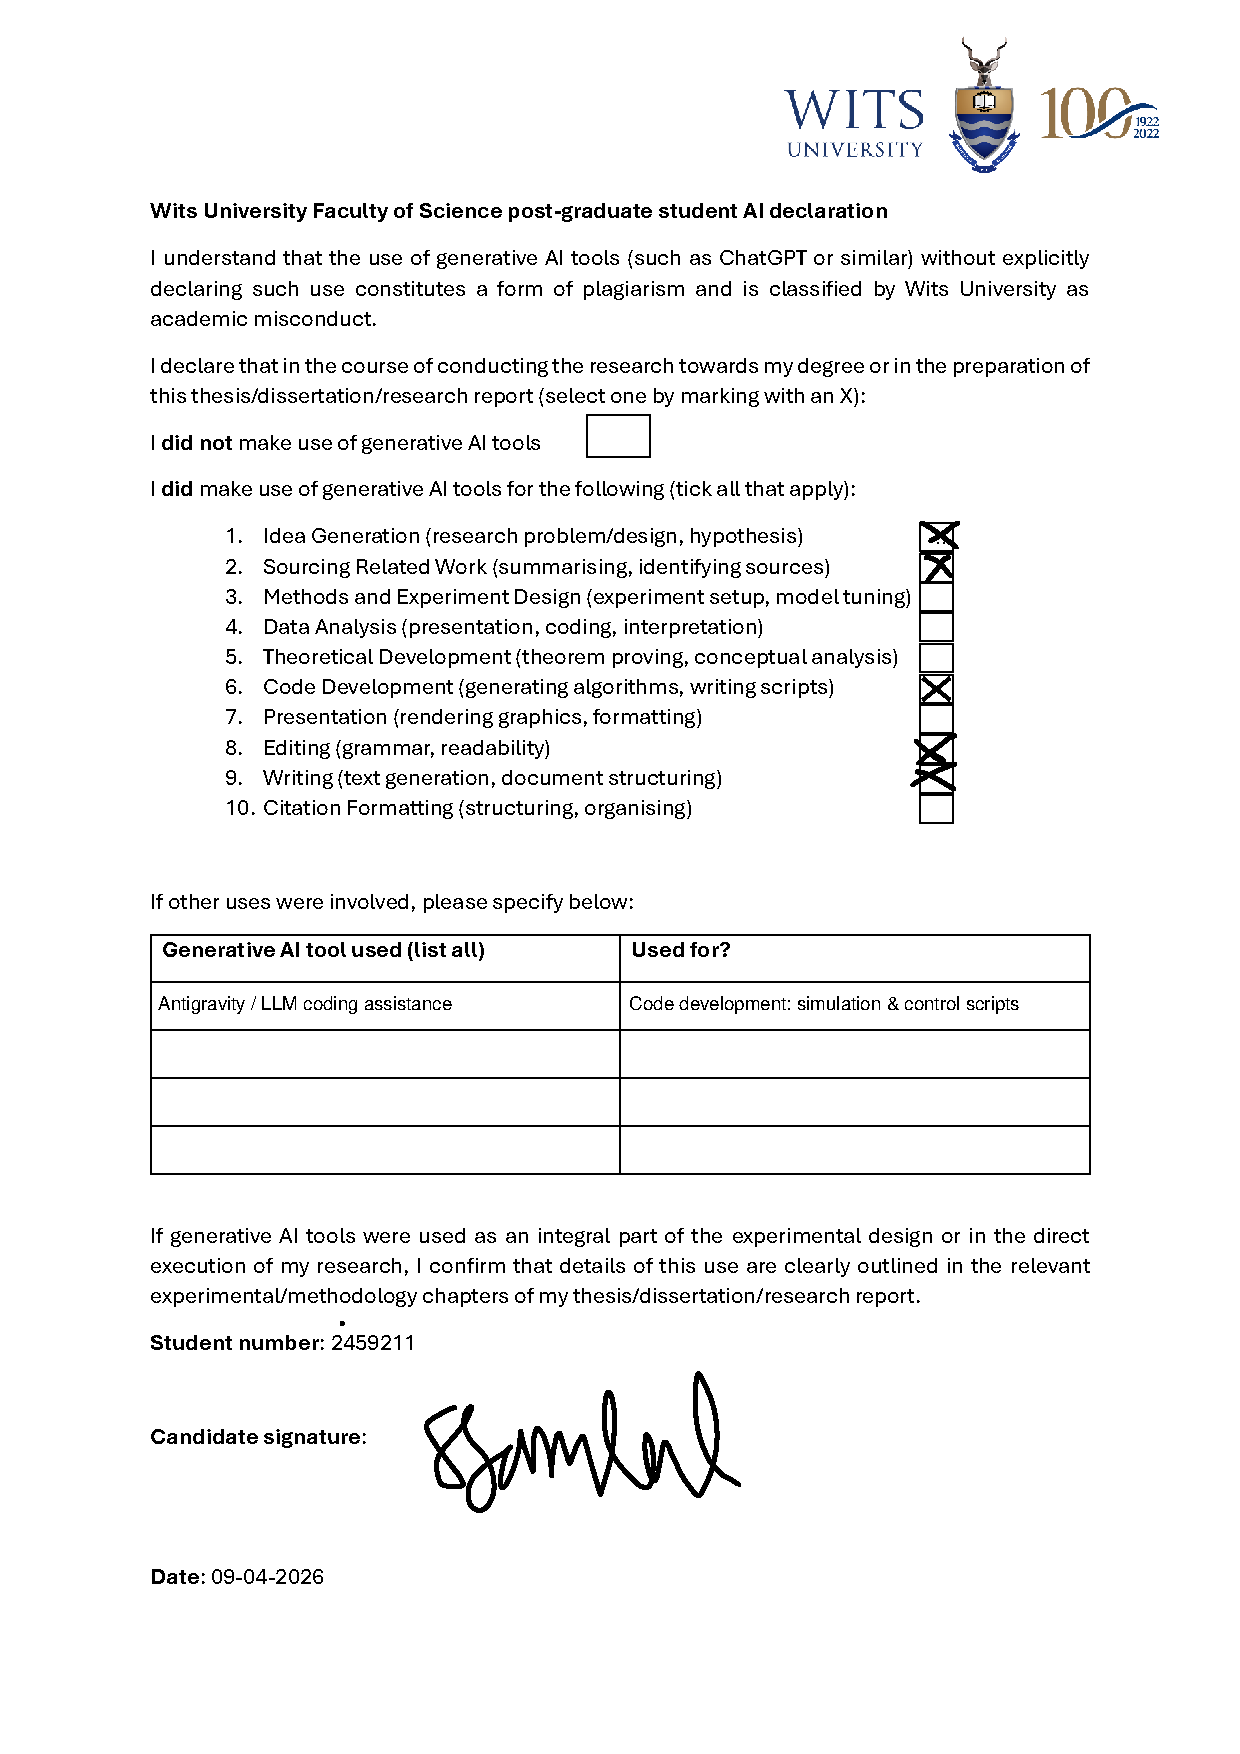
\includepdf[pages=-]{declaration.pdf}
\end{document}
